\documentclass[t]{beamer}
\mode<presentation>

\usepackage{etex}

\usetheme{Madrid}
% other themes: Warsaw, AnnArbor, Antibes, Bergen, Berkeley, Berlin, Boadilla, boxes, CambridgeUS, Copenhagen, Darmstadt, default, Dresden, Frankfurt, Goettingen,
% Hannover, Ilmenau, JuanLesPins, Luebeck, Madrid, Maloe, Marburg, Montpellier, PaloAlto, Pittsburg, Rochester, Singapore, Szeged, classic

\setbeamertemplate{navigation symbols}{\insertslidenavigationsymbol}

\usecolortheme{dolphin}
%\usecolortheme{seagull}
% color themes: albatross, beaver, beetle, crane, default, dolphin, dov, fly, lily, orchid, rose, seagull, seahorse, sidebartab, structure, whale, wolverine

%\usefonttheme{serif}
% font themes: default, professionalfonts, serif, structurebold, structureitalicserif, structuresmallcapsserif

% pdf is displayed in full screen mode automatically
%\hypersetup{pdfpagemode=FullScreen}

%\AtBeginSection[]
%{
%  \begin{frame}<beamer>
%    \frametitle{Outline}
%    \tableofcontents[currentsection,currentsubsection]
%  \end{frame}
%}

% define your own colours:
\definecolor{Red}{rgb}{1,0,0}
\definecolor{Blue}{rgb}{0,0,1}
\definecolor{Green}{rgb}{0,1,0}
\definecolor{magenta}{rgb}{1,0,.6}
\definecolor{lightblue}{rgb}{0,.8,1}
\definecolor{lightpurple}{rgb}{.6,.4,1}
\definecolor{gold}{rgb}{.6,.5,0}
\definecolor{orange}{rgb}{1,0.4,0}
\definecolor{hotpink}{rgb}{1,0,0.5}
\definecolor{newcolor2}{rgb}{.5,.3,.5}
\definecolor{newcolor}{rgb}{0,.3,1}
\definecolor{newcolor3}{rgb}{1,0,.35}
\definecolor{darkgreen1}{rgb}{0, .35, 0}
\definecolor{darkgreen}{rgb}{0, .6, 0}
\definecolor{darkred}{rgb}{.75,0,0}

\xdefinecolor{olive}{cmyk}{0.64,0,0.95,0.4}
\xdefinecolor{purpleish}{cmyk}{0.75,0.75,0,0}

%\usepackage{beamerinnerthemerounded}
% inner themes include circles, default, inmargin, rectangles, rounded

%\usepackage{beamerouterthemesmoothbars}
% outer themes include default, infolines, miniframes, shadow, sidebar, smoothbars, smoothtree, split, tree

\useoutertheme[subsection=false]{smoothbars}

% to have the same footer on all slides
\setbeamertemplate{footline}[text line]{
\raisebox{3pt}{
\includegraphics[height=15pt]{su-long.eps}}\hfill 
\raisebox{5pt}{Math 207:  Statistics}\hfill 
\raisebox{5pt}{Probability}\hfill
\raisebox{5pt}{\insertframenumber/\pageref{lastpage}}}
%\setbeamertemplate{footline}[text line]{} % or empty footer

% include packages
\usepackage{subfigure}
\usepackage{multicol}
\usepackage{amsmath}
\usepackage{epsfig}
\usepackage{graphicx}
\usepackage[all,knot]{xy}
\xyoption{arc}
\usepackage{url}
\usepackage{multimedia}
\usepackage{hyperref}
\usepackage{setspace}

\title{Math 207:  Statistics}
\subtitle{What Are the Chances?}
\author{Ralph Wojtowicz}
\institute{Mathematics Department\\ Shenandoah University}
%\date{\scriptsize 17 February 2012}

\usepackage{pstricks,pst-grad,pst-func,pst-text,pst-node,multido,pst-plot,calc,pst-3dplot}

\newcommand{\BRACE}{
\begin{pspicture}(-3,-2.1)(3,1.1)
\psset{yunit=3,linewidth=0.02}
\psline(-3.5,0)(3.5,0)  
  \psline(-3,0)(-3,-0.04) \rput[t](-3,-0.07){\scriptsize -3\hphantom{-}}
  \psline(-2,0)(-2,-0.04) \rput[t](-2,-0.07){\scriptsize -2\hphantom{-}}
  \psline(-1,0)(-1,-0.04) \rput[t](-1,-0.07){\scriptsize -1\hphantom{-}}
  \psline(0,0)(0,-0.04)   \rput[t](0,-0.07){\scriptsize 0}
  \psline(1,0)(1,-0.04)   \rput[t](1,-0.07){\scriptsize 1}
  \psline(2,0)(2,-0.04)   \rput[t](2,-0.07){\scriptsize 2}
  \psline(3,0)(3,-0.04)   \rput[t](3,-0.07){\scriptsize 3}
  \rput[l](3.6,0){\scriptsize $x$}
\psline(0,0)(0,0.5)
  \psline(-0.12,0.5)(0,0.5)    \rput[r](-0.21,0.5){\scriptsize $0.5$}
  \psline(-0.12,0.25)(0,0.25)  \rput[r](-0.21,0.25){\scriptsize $0.25$}
\psGauss[linecolor=blue,linewidth=0.02,sigma=1,mue=0]{-3}{3}
\pnode(-1,-0.15){A}\pnode(1,-0.15){B}
\psbrace[braceWidth=0.02,braceWidthInner=5pt,braceWidthOuter=5pt](A)(B){\rput{90}(0.25,-0.05){\scriptsize 68\%}}
%
\pnode(-2,-0.15){C}\pnode(2,-0.15){D}
\psbrace[braceWidth=0.02,braceWidthInner=25pt,braceWidthOuter=5pt](C)(D){\rput{90}(0.25,-0.05){\scriptsize 95\%}}
%
\pnode(-3,-0.15){E}\pnode(3,-0.15){F}
\psbrace[braceWidth=0.02,braceWidthInner=45pt,braceWidthOuter=5pt](E)(F){\rput{90}(0.25,-0.1){\scriptsize 99.7\%}}
\end{pspicture}}

\begin{document}

%\frame[plain]{
%	\titlepage
%}


\begin{frame}[plain]
\definecolor{myblue}{rgb}{0,0,0.6}
\definecolor{grayA}{rgb}{0.95,0.95,0.95}
\definecolor{grayB}{rgb}{0.98,0.98,0.98}
\begin{center}

%\begin{pspicture}(0,0)(7,4.8)
\begin{pspicture}(-6,-7)(6,2)
\rput(0,-1.85){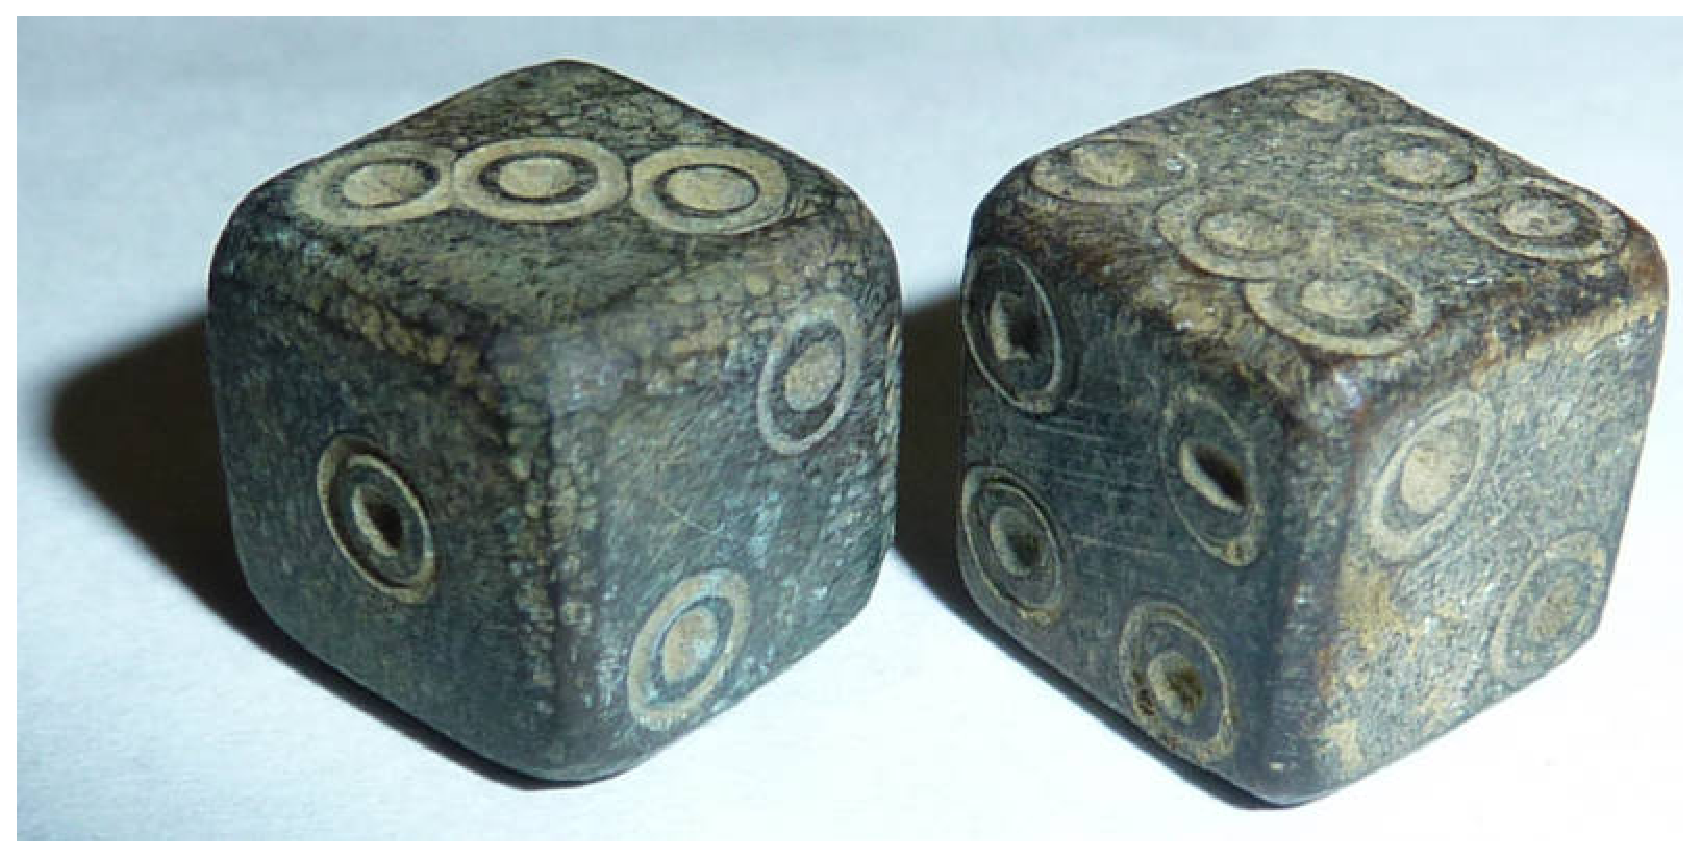
\includegraphics[height=4.2cm]{dice.eps}}
\psframe[linewidth=0.02,linecolor=gray](-6.2,-7)(6.2,2.2)
\psframe[linewidth=0.02,linecolor=gray](-6.15,-6.95)(6.15,2.15)
\rput(0,1.4){\color{myblue}\large Math 207:  Statistics}
\rput(0,0.6){\color{myblue}What Are the Chances?}
%\psframebox(0,0)(4,4)
\rput(0,-4.4){\scriptsize Dr.~Ralph Wojtowicz}
\rput(0,-4.9){\scriptsize Mathematics Department}
\rput(0,-5.7){
\includegraphics[height=1cm]{su-long.eps}}
%
%\rput(0,-6.5){\scriptsize 17 February 2012}
\end{pspicture}
\end{center}

\end{frame}

%\section[Outline]{}

\addtocounter{page}{-1}
\addtocounter{framenumber}{-1}

{\footnotesize
\frame{\tableofcontents}
}

\section{Probability}
\subsection{Probability}
\begin{frame}[t]\frametitle{Probability}
{\footnotesize
\begin{itemize}
\item The \textbf{probability (chance)} of something gives the percentage
of time it is expected to happen, when the basic process is 
repeated independently and under the same conditions. This is the \textit{frequency theory} of probability.
\item Probabilities are between $0$ and $1$:  $0\%\leq P(\mbox{event})\leq 100\%$.
\item If an event is impossible, its chance is 0\%.
\item If an event is sure to happen, its chance is 100\%.
\item $P(\mbox{event})= 100\%\;-\;P(\mbox{event will not occur})$
\item Examples
  \begin{itemize} 
   \item \footnotesize Flip a fair coin:  $P(H)=1/2=50\%$.
   \item \footnotesize Roll a balanced die:  $P(5)=1/6\approx 16.7\%$.
   \item \footnotesize A box contains 3 red marbles and 2 blue ones.  One marble is drawn at random 
      $P(\mbox{red}) = 3/5 = 0.6 = 60\%$ and $P(\mbox{blue}) = 100\% - 60\% = 40\%$.
%   \item item
  \end{itemize}
\item {\color{blue}Box models}:   In a random  draw, all tickets have the 
same chance to be picked.
\end{itemize}
\begin{center}
\begin{pspicture}(0,0.3)(5,0.8)
\psline(-0.1,1)(-0.1,0)(5.1,0)(5.1,1)
\psframe(0.1,0.1)(0.9,0.9)\rput(0.5,0.5){1}
\psframe(1.1,0.1)(1.9,0.9)\rput(1.5,0.5){2}
\psframe(2.1,0.1)(2.9,0.9)\rput(2.5,0.5){3}
\psframe(3.1,0.1)(3.9,0.9)\rput(3.5,0.5){4}
\psframe(4.1,0.1)(4.9,0.9)\rput(4.5,0.5){5}
\end{pspicture}
\end{center}
%\begin{itemize}
%\item Drawing with and without replacement
%\end{itemize}
}
\end{frame}

\section{Conditional Probability}
\subsection{Conditional Probability}
\begin{frame}[t]\frametitle{Conditional Probability}
{\footnotesize
\begin{itemize}
\item Given two events $A$ and $B$, the \textbf{conditional probability
of $A$ given $B$} is the probability that $A$ 
{\color{blue}\textbf{will}} occur given that
one knows that $B$ {\color{blue}\textbf{did}} occur.
\item Notation $P(A\,\vert\,B)$
\item Examples:
   \begin{itemize}
   \item \footnotesize $P(\mbox{die roll is a 4}\;\vert\,\mbox{the die roll is even}) = 1/3$\\[3pt]
   \item \footnotesize $P(\mbox{die roll is a 3}\;\vert\,\mbox{the die roll is even}) = 0$\\[3pt]
   \item \footnotesize $P(\mbox{blackjack on second card drawn}\;\vert\,\mbox{first card drawn is ace}) = 
        16/51$\\ (What else is assumed here?)\\[3pt]
   \item \footnotesize $P(\mbox{heads on 2nd coin flip}\,\vert\,\mbox{heads on first})
       =1/2$.\\[3pt]
   \item \footnotesize $P(\mbox{$4$ on second draw if you put the first ticket back}\;\vert\;
     \mbox{$1$ on first draw})=1/5$.\\
%
    $P(\mbox{$4$ on second draw without replacement}\;\vert\;
        \mbox{$1$ on first draw})=1/4$.
   \end{itemize}
\end{itemize}
\begin{center}
\begin{pspicture}(0,0.3)(5,0.7)
\psline(-0.1,1)(-0.1,0)(5.1,0)(5.1,1)
\psframe(0.1,0.1)(0.9,0.9)\rput(0.5,0.5){1}
\psframe(1.1,0.1)(1.9,0.9)\rput(1.5,0.5){2}
\psframe(2.1,0.1)(2.9,0.9)\rput(2.5,0.5){3}
\psframe(3.1,0.1)(3.9,0.9)\rput(3.5,0.5){4}
\psframe(4.1,0.1)(4.9,0.9)\rput(4.5,0.5){5}
\end{pspicture}
\end{center}
\begin{itemize}
\item $P(\mbox{third card drawn is Q$\heartsuit$}\;\vert\; \mbox{no information about first two cards}) = 1/52$.
\end{itemize}
}
\end{frame}

\section{Multiplication Rule}
\subsection{Multiplication Rule}
\begin{frame}[t]\frametitle{Multiplication Rule}
{\small
\begin{itemize}
\item \textbf{Multiplication Rule}:  The probability that two 
things will both occur equals the probability that the first
will occur times the probability that the second will occur
given first  did occur.
\[{\color{blue}P(\mbox{$A$ and $B$}) = P(A)\,P(B\,\vert\,A)}
  \hspace{10pt}   \mbox{\footnotesize (assuming $A$ is possible)}\vspace{-4pt}\]
\item Examples:
   \begin{itemize}
   \item $P(\mbox{draw two aces in a row}) = \frac{4}{52}\,\frac{3}{51}$\\[3pt]
   \item $P(\mbox{head followed by tail}) = \frac{1}{2}\,\frac{1}{2}$.\\[3pt]
   \item $P(\mbox{4 followed by odd number}) = \frac{1}{5}\,\frac{3}{4}$
        \hspace{5pt} {\footnotesize(box below without~replacement)}\\[3pt]
   $P(\mbox{4 followed by odd number}) = \frac{1}{5}\,\frac{3}{5}$
        \hspace{5pt} {\footnotesize(box below with~replacement)}
\begin{center}
\begin{pspicture}(0,-0.1)(5,1.0)
\psline(-0.1,1)(-0.1,0)(5.1,0)(5.1,1)
\psframe(0.1,0.1)(0.9,0.9)\rput(0.5,0.5){1}
\psframe(1.1,0.1)(1.9,0.9)\rput(1.5,0.5){2}
\psframe(2.1,0.1)(2.9,0.9)\rput(2.5,0.5){3}
\psframe(3.1,0.1)(3.9,0.9)\rput(3.5,0.5){4}
\psframe(4.1,0.1)(4.9,0.9)\rput(4.5,0.5){5}
\end{pspicture}
\end{center}
%
\item $P(\mbox{three tails in a row}) = \frac{1}{2}\,\frac{1}{2}\,\frac{1}{2}= \frac{1}{8}$\\[5pt]
\item $P(\mbox{three face cards in a row}) = \frac{12}{52}\,\frac{11}{51}\,\frac{10}{50}$
   \end{itemize}
\end{itemize}
}
\end{frame}

%\section{Independence}
\subsection{Independence}
\begin{frame}[t]\frametitle{Independence}
{\small
\begin{itemize}
\item Two events $A$ and $B$ are 
    \textbf{independent} if the probability 
   of $A$ given $B$ is equal to the probability of $A$ (without
   knowledge of $B$).  Otherwise, the events are \textbf{dependent}.
\item Formula:  $A$ and $B$ are independent if $P(A\,\vert\,B)=P(A)$
\item Examples of independent events:%\vspace{-2pt}
   \begin{itemize}
    \item Outcomes of two coin flips.\\[2pt]
    \item Even on first die roll, odd on second\\[2pt]
    \item Draws from a box with replacement.
   \end{itemize}
\item Examples of dependent events:%\vspace{-3pt}
   \begin{itemize}
    \item Draws from a box without replacement.\\[3pt]
    \item $A=\mbox{a randomly selected subject is over 6' tall}$\\ $B=\mbox{the father of a randomly selected
      subject is over 6' tall}$\\[3pt]
    \item $A=\mbox{IBM stock price will increase next week}$\\ $B=\mbox{Google stock price will increase next week}$
   \end{itemize}
\end{itemize}
}
\end{frame}

\section{Addition Rule}
\subsection{Addition Rule}
\begin{frame}
\frametitle{Addition Rule}
{\small
\begin{itemize}
\item \textbf{Addition Rule}:  The probability that at least one of two 
things will both  equals the probability that the first
will occur plus the probability that the second will occur minus the chance that both will occur
\[\color{blue}P(\mbox{$A$ or $B$}) = P(A) \; + \; P(B) \; - \; \,P(\mbox{$A$ and $B$})\vspace{-4pt}\]
\item Examples:
   \begin{itemize}
   \item \footnotesize $P(\mbox{draw a $\heartsuit$ or a 10}) = \frac{13}{52} + \frac{4}{52} - \frac{1}{52}$\\[5pt]
   \item \footnotesize $P(\mbox{draw a $\heartsuit$ or a $\clubsuit$}\;) = \frac{13}{52} + \frac{13}{52} - 0$\\[5pt]
   \item \footnotesize Roll two dice:  $P(\mbox{sum is less than 6}\; \mbox{or}\; \mbox{roll is doubles}) = 
           \frac{10}{36} + \frac{6}{36} - \frac{2}{36}$\\[5pt]
   \item \footnotesize Flip 10 coins:  $P(\mbox{at least 9 tails}) = P(\mbox{9 tails}) \; + \; P(\mbox{10 tails}) \; - \; 0$.  
   \end{itemize}
\end{itemize}}

\end{frame}

\subsection{Mutually Exclusive Events}
\begin{frame}
\frametitle{Mutually Exclusive Events}

{\small
\begin{itemize}
\item Two events $A$ and $B$ are \textbf{mutually exclusive} when the occurrence of one
  prevents the occurrence of the other:  one excludes the other.
\item If $A$ and $B$ are mutually exclusive, then \\[-2pt]
  \begin{itemize}
   \item \footnotesize $P(A\;\mbox{and}\; B)=0$\\[3pt]
   \item \footnotesize $P(A\;\mbox{or}\; B) = P(A)\; + \; P(B)$\vspace{-2pt}
   \end{itemize}
\item Examples of mutually exclusive events:
  \begin{itemize}
  \item \footnotesize $A=\mbox{first card is a 10}$ and $B=\mbox{first card is a 7}$\\[3pt]
  \item \footnotesize $A=\mbox{Apple stock price will have a net increase next week}$\\
                       $B=\mbox{Apple stock price will have a net decrease next week}$\\[3pt]
  \item \footnotesize $A=\mbox{out of 10 coin flips, exactly 3 are H}$ and
$B=\mbox{out of 10 coin flips, exactly 5 are H}$
  \end{itemize}
\item Examples of events that are not mutually exclusive:
  \begin{itemize}
  \item \footnotesize $A=\mbox{first card is a 10}$ and $B=\mbox{first card is a $\heartsuit$}$\\[3pt]
  \item \footnotesize $A=\mbox{Apple stock will increase next week}$ and $B=\mbox{IBM stock will decrease next week}$
  \end{itemize}
\end{itemize}
}
\end{frame}

\section{Binomial Formula}
\subsection{Examples to Motivate Use of the Binomial Formula}
\begin{frame}
\frametitle{Examples to Motivate Use of the Binomial Formula}
{\small
\begin{itemize}
\item A coin is tossed four times.  What is the chance of getting exactly one head?
   \begin{itemize}
   \item \footnotesize List the possibilities:  HTTT or THTT or TTHT or TTTH.\\[3pt]
   \item \footnotesize By the multiplication rule, each possibility has chance $(1/2)^4=1/16$.\\[3pt]
   \item \footnotesize By the addition rule, the final answer is $\frac{1}{16}+\frac{1}{16}+\frac{1}{16}+\frac{1}{16} 
       = 4\left(\frac{1}{16}\right)=\frac{1}{4}$\\[3pt]
   \end{itemize}
\item A coin is tossed 5 times.  What is the chance of getting exactly two heads?
   \begin{itemize}
   \item \footnotesize List the possibilities:  HHTTT or HTHTT or HTTHT or HTTTH or THHTT or THTHT or THTTH or TTHHT
            or TTHTH or TTTHH.\\[3pt]
   \item \footnotesize By the multiplication rule, each possibility has chance $(1/2)^5=1/32$.\\[3pt]
   \item \footnotesize By the addition rule, the final answer is $10\left(\frac{1}{32}\right)\;=31.25\%$\\[3pt]
   \end{itemize}
\item A coin is tossed 20 times.  What is the chance of getting exactly 10 heads?
   \begin{itemize}
   \item \footnotesize There are 184,756 possibilities but we don't want to list them!\\[3pt]
   \item \footnotesize The chance of each is $(1/2)^{20}$.\\[3pt]
   \item \footnotesize  So, the final answer is $184,\!756\left(\frac{1}{2}\right)^{20}\;\approx\;17.6\%$.
   \end{itemize}
\end{itemize}}
\end{frame}

\subsection{Binomial Formula}
\begin{frame}
\frametitle{Binomial Formula}
{\footnotesize
\begin{itemize}
\item Factorials:  $n!=n\times (n-1)\times (n-2)\times \cdots \times 2 \times 1$\vspace{-2pt}
  \begin{itemize}
  \item \footnotesize Examples:\\
       $5!=5\times 4\times 3\times 2\times 1 = 120$\\
       $4!=4\times 3\times 2\times 1 = 24$\\
       and $0! = 1! = 1$ by definition
  \end{itemize}
\item The chance that an event will occur exactly $k$ times out of $n$ is given by the 
\textbf{binomial formula}:\vspace{-3pt}
\[\frac{n!}{k!\;(n-k)!}\; p^k\; (1-p)^{n-k}\vspace{3pt}\]
where $n$ is the number of trials, $k$ is the number of times the event is to occur, and
$p$ is the probability that the event will occur on any particular trial
\item The factorial term counts all the possibilities (addition rule) while the rest of the formula
    gives the chance of each individual possibility (multiplication rule).
\item Assumptions:\vspace{-1pt}
  \begin{itemize}
  \item \footnotesize The value $n$ must be fixed in advance.
  \item \footnotesize $p$ must be the same from trial to trial.
  \item \footnotesize The trials must be independent.
  \end{itemize}
\end{itemize}
}
\end{frame}

\subsection{Binomial Formula Examples}
\begin{frame}
\frametitle{Binomial Formula Examples}
{\small
\begin{itemize}
\item A coin is tossed four times.  What is the chance of getting exactly one head?\\
    \begin{itemize}
    \item \footnotesize $n=4$, $k=1$ and $p=1/2$\vspace{-4pt}
{\scriptsize\begin{align*}
\frac{4!}{1!\,(4-1)!}\,(1/2)^1\;(1/2)^{4-1} &= \frac{4\cdot 3\cdot 2\cdot 1}{1\cdot 3!}\,(1/2)\,(1/2)^3\\[2pt]
           & = \frac{4\cdot 3\cdot 2\cdot 1}{3\cdot 2\cdot 1}\,(1/2)^4\\[2pt] & =4\,(1/16)=1/4
\end{align*}}
    \end{itemize}
\item A coin is tossed 5 times.  What is the chance of getting exactly two heads?
    \begin{itemize}
    \item \footnotesize $n=5$, $k=2$ and $p=1/2$\\[2pt]
    \item \scriptsize $\displaystyle\frac{5!}{2!\,3!}\,(1/2)^2\,(1/2)^3 = \frac{5\cdot 4\cdot 3\cdot 2\cdot 1}{2\cdot 3\cdot 2}\,(1/2)^5 = 10\,(1/2)^5$
    \end{itemize}
\item A box has 4 red marbles and 5 green ones.  Ten marbles are drawn at random with replacement.
   What is the chance that exactly 2 are green?
  \begin{itemize}
  \item \footnotesize $n=10$, $k=2$ and $p=5/9$.\\[2pt]
  \item \footnotesize Answer $= 45\,(5/9)^2\,(4/9)^8$
  \end{itemize}
\end{itemize}
}
\label{lastpage}
\end{frame}
\end{document}
